%%%%%%%%%%%%%%%%%%%%%%%%%%%%%%%%%%%%%%%%%
% Fancyslides Presentation
% LaTeX Template
% Version 1.0 (30/6/13)
%
% This template has been downloaded from:
% http://www.LaTeXTemplates.com
%
% The Fancyslides class was created by:
% Paweł Łupkowski (pawel.lupkowski@gmail.com)
%
% License:
% CC BY-NC-SA 3.0 (http://creativecommons.org/licenses/by-nc-sa/3.0/)
%
%%%%%%%%%%%%%%%%%%%%%%%%%%%%%%%%%%%%%%%%%

%----------------------------------------------------------------------------------------
%	PACKAGES AND OTHER DOCUMENT CONFIGURATIONS
%----------------------------------------------------------------------------------------

\documentclass{fancyslides}
%\documentclass[aspectratio=169]{beamer}
\usepackage[utf8]{inputenc} % Allows the usage of non-english characters

%\usepackage{fontspec}
%\setmainfont{Vera}

\usepackage{booktabs} % Allows the use of \toprule, \midrule and \bottomrule in tables
\graphicspath{{images/}} % Location of the slide background and figure files
\usepackage{soul}
\usepackage{xcolor}
\usepackage{helvet}
\usepackage{graphicx}
\usepackage{lmodern}
\usepackage[]{hyperref,graphicx,siunitx,lmodern,booktabs,tikz,tensor}
\usepackage{pgfplots, pgfplotstable}
\usepackage{tikz}
\usepackage{pdfpc-commands}
\usepackage[mode=buildnew]{standalone}
% Beamer options - do not change
\usetheme{default} 
\setbeamertemplate{navigation symbols}{} % Disable the slide navigation buttons on the bottom of each slide
%\setbeamercolor{structure}{fg=\yourowntexcol} % Define the color of titles and fixed text elements (e.g. bullet points)
\setbeamercolor{normal text}{fg=\yourowntexcol} % Define the color of text in the presentation
\tikzstyle{math}=[execute at begin node={$\displaystyle}, execute at end node={$}]
%------------------------------------------------
% COLORS
% The following colors are predefined in this class: white, black, gray, blue, green and newhopeblue

% Define your own color as follows:
\definecolor{pink}{rgb}{156,0,151}
\definecolor{amber}{rgb}{255,194,0}
\newcommand{\structureopacity}{1} % Opacity (transparency) for the structure elements (boxes and circles)

\newcommand{\strcolor}{newhopeblue} % Set the color of structure elements (boxes and circles)
\newcommand{\yourowntexcol}{white} % Set the text color

%----------------------------------------------------------------------------------------
%	TITLE SLIDE
%----------------------------------------------------------------------------------------

\newcommand{\titlephrase}{Photometric Analysis of Meteoritic Fireballs} % Presentation title
\newcommand{\name}{Luke Galbraith Russell} % Presenter's name
\newcommand{\affil}{Willamette University} % Presenter's institution
\newcommand{\email}{$<$lgrussel$>$} % Presenter's email address

\begin{document}

%\startingslide % This command inserts the title slide as the first slide

%----------------------------------------------------------------------------------------
%	PRESENTATION SLIDES
%----------------------------------------------------------------------------------------

\fbckg{skypic1.png} % Slide background image
\begin{frame}
%\begin{alertenv}

%\begin{center}
%\textcolor{white}{\Huge Photometric Analysis of \\ Meteoritic Fireballs}
%\end{center}
\begin{center}
	
\includegraphics[scale=.23]{title.png}
\end{center}

\begin{center}
\textcolor{newhopeblue}{\Large \textbf{Luke Galbraith Russell} $\bullet$ \textbf{Willamette University}}
\end{center}
\end{frame}


%------------------------------------------------
%  slide3
%------------------------------------------------

\fbckg{2.jpg} % Slide background image
\begin{frame}
	\pgfsetfillopacity{.75}
	\framedsl{Satellites Entering orbit}
	\pgfsetfillopacity{1}
	%\begin{center}
		\begin{tikzpicture}[remember picture, overlay]
			\node[font=\bf\Huge] at (2,2) {2006};
			\node[font=\bf\Huge] at (2,0) {2017};
			\node[font=\bf\Huge] at (2,-2) {2022};
			\node<1> at (11,2){
\includegraphics[height=1.25cm]{satlabel.png}};
			\node[font=\bf\normalsize] at (11.55,2.20) {50};
			\node[font=\bf\large] at (11.55,1.8) {satellites};
			%\node[font=\bf\large] at (11.75,1.05) {launched};
			\node[white] at (4,2) {
\includegraphics[width=1cm]{satt.pdf}};
			\foreach \x in {4,5,...,7} \node[white] at (\x,0) {
\includegraphics[width=1cm]{satt.pdf}};

			\foreach \x in {4,5,...,12} \node[white] at (\x,-2) {
\includegraphics[width=1cm]{satt.pdf}};

			\foreach \x in {2,3,...,10} \node[white] at (\x+2,-3) {
\includegraphics[width=1cm]{satt.pdf}};
		\end{tikzpicture}
\end{frame}
%------------------------------------------------
% slide 2
%------------------------------------------------
\fbckg{2.jpg}
\begin{frame}
\pgfsetfillopacity{.75}
\framedsl{Near-Earth Objects}
\pgfsetfillopacity{1}
	\begin{center}
	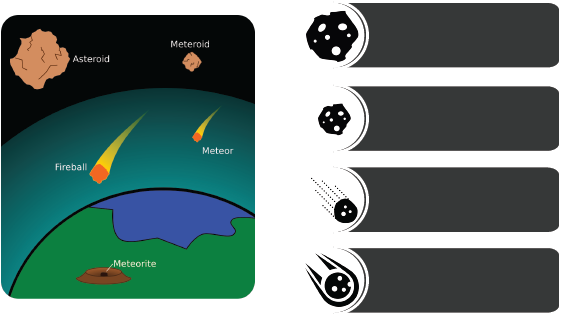
\includegraphics[width=\linewidth, height = 200pt]{meteorslide.png}
	\end{center}
	\begin{tikzpicture}[remember picture, overlay]
		%\node at (0,0) {includegraphics[width=.8linewidth]{chain.png}}
		\node[font=\bf\large] at (11.5,6.95) {large rock in orbit};
		\node[font=\bf\large] at (11.5,5.15) {small rock in orbit};
		\node[font=\bf\normalsize] at (11.5,3.5) {small rock };
		\node[font=\bf\normalsize] at (11.5,3) {entering atmosphere};
		\node[font=\bf\normalsize] at (11.5,1.75) {large rock };
		\node[font=\bf\normalsize] at (11.5,1.25) {entering atmosphere};
	\end{tikzpicture}

%\center
%\begin{tikzpicture}[remember picture, overlay]
		%\node<1> at (0,-.5){\includegraphics[width=.3\linewidth]{fireball.png}};
		%\node<1> at (-6.5,-1){
\includegraphics[width=.15\linewidth]{category.png}};
		%\node<1> at (-4,-1){
\includegraphics[width=.15\linewidth]{category.png}};
		%\node<1> at (6.5,-1){
\includegraphics[width=.15\linewidth]{category.png}};
		%\node<1> at (4,-1){
\includegraphics[width=.15\linewidth]{category.png}};

		%\node<1> at (-4.5,0){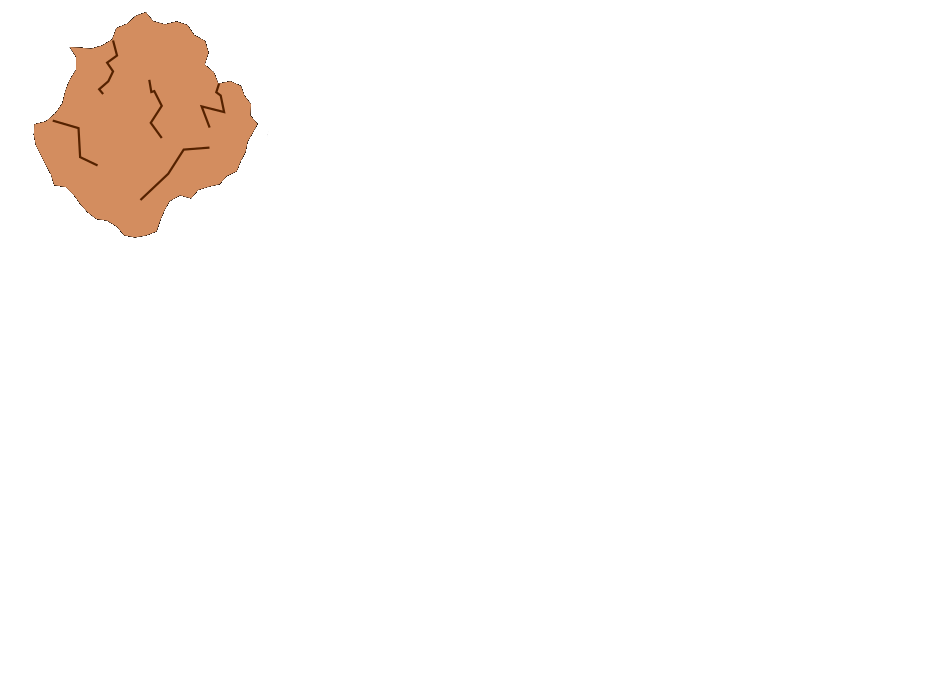
\includegraphics[width=.4\linewidth]{asteroid.png}};
		%\node<1> at (-5.3,0){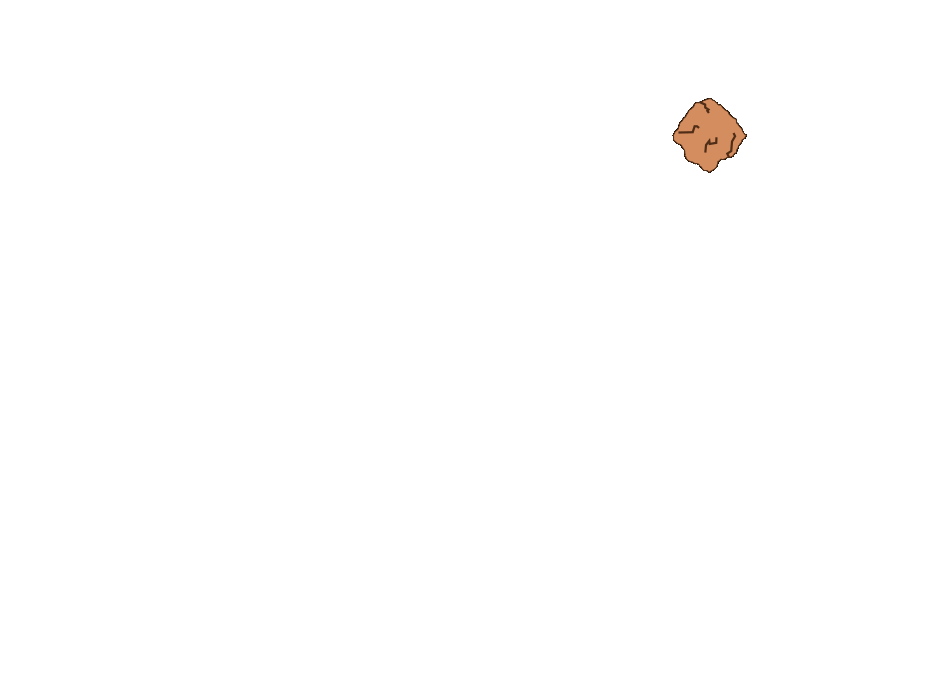
\includegraphics[width=.4\linewidth]{meteoroid.png}};
		%\node<1> at (5.1,3.5){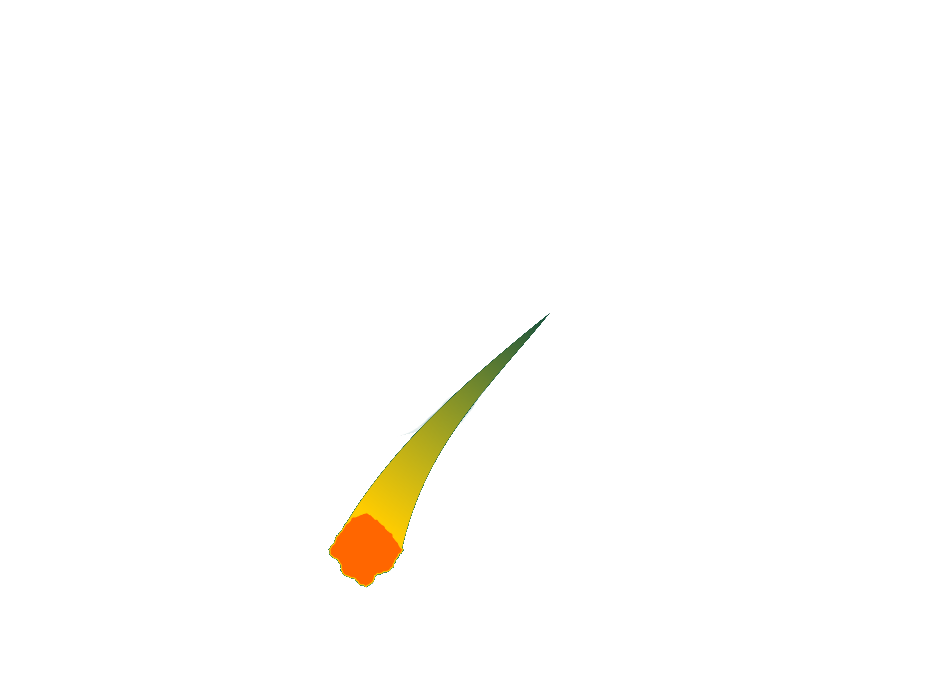
\includegraphics[width=.8\linewidth]{meteor.png}};
		%\node<1> at (7.2,2.4){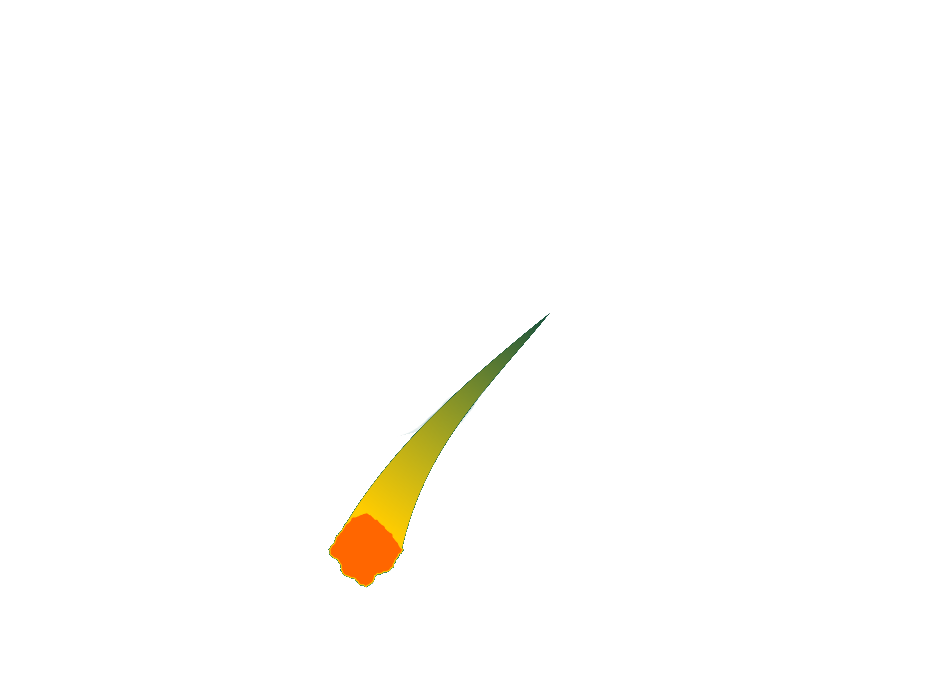
\includegraphics[width=.4\linewidth]{meteor.png}};

%\end{tikzpicture}
\end{frame}



\fbckg{2.jpg}
\begin{frame}
\pgfsetfillopacity{.75}
\framedsl{Near-Earth Objects}
\pgfsetfillopacity{1}
	\begin{center}
	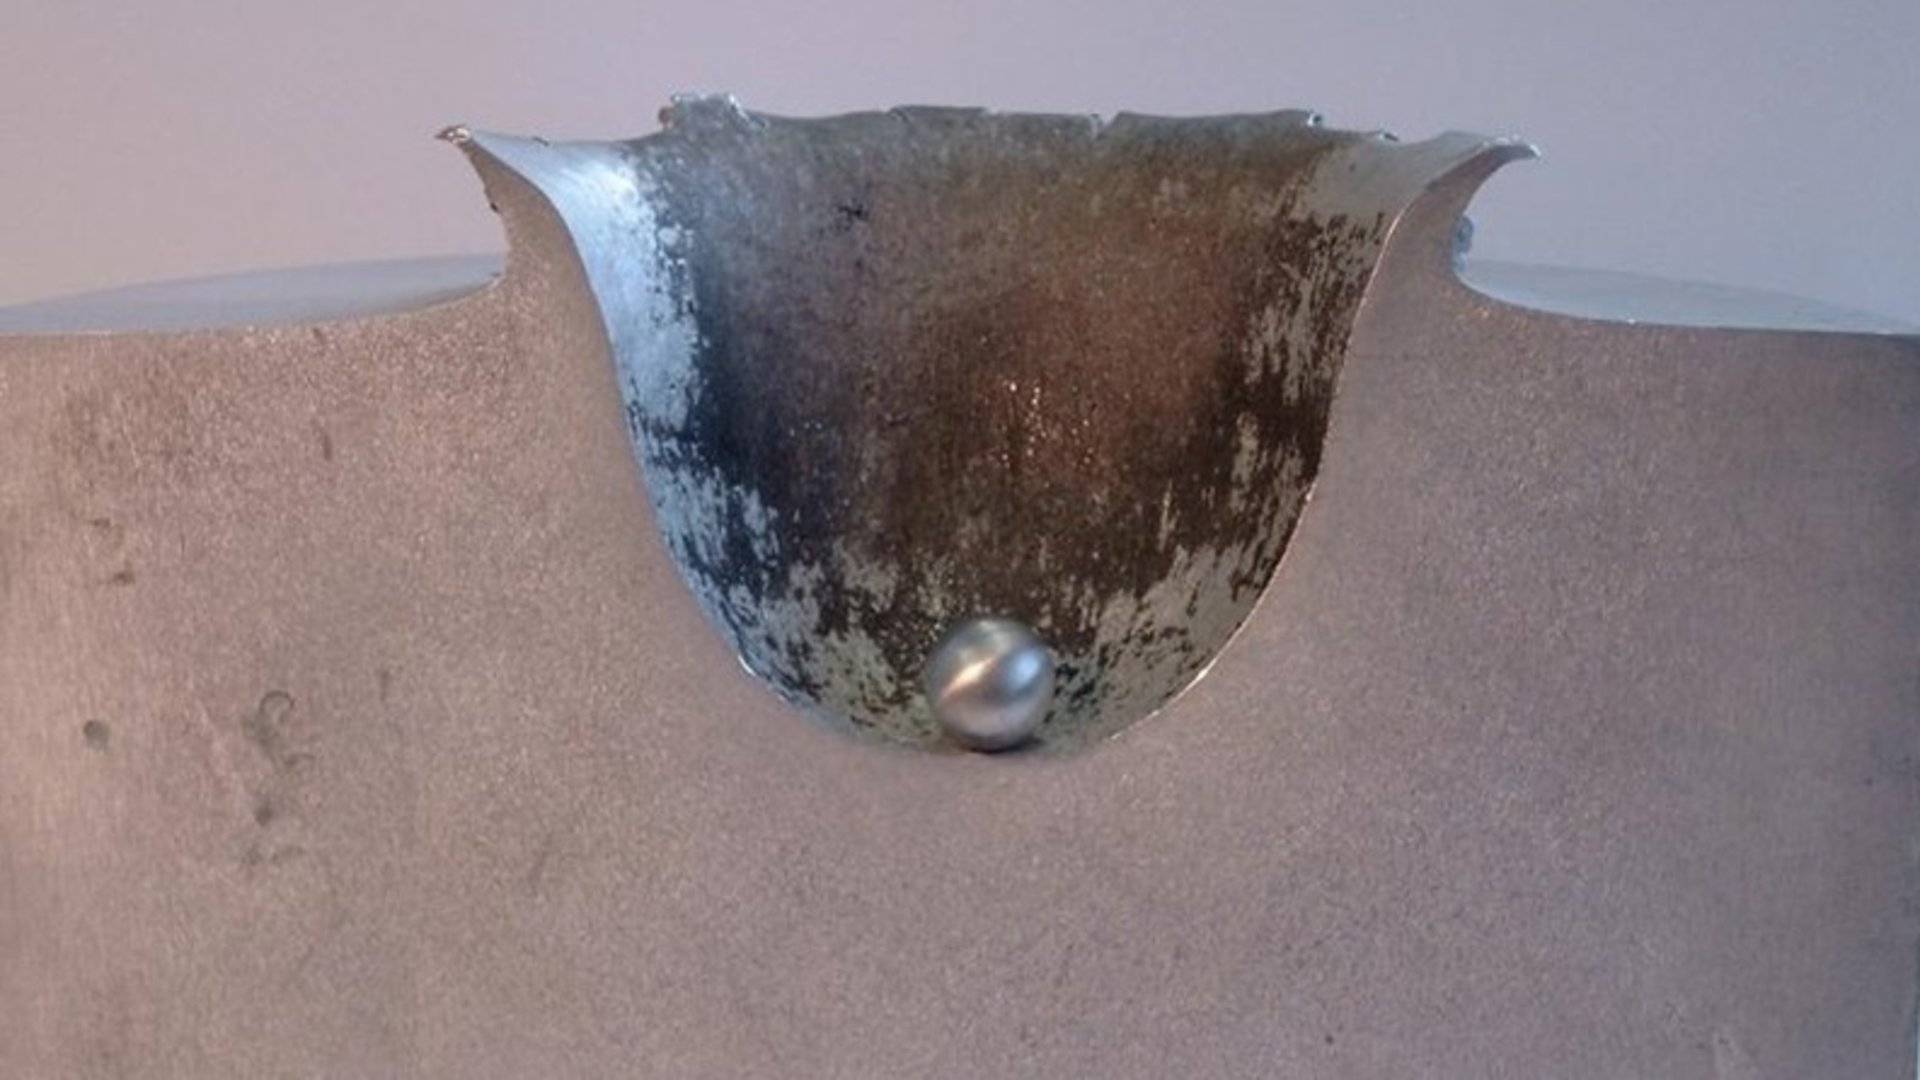
\includegraphics[height = 160pt]{damage.jpg}
	\end{center}
	\begin{tikzpicture}[remember picture, overlay]
		\node<1> at (2.3,.75){
\includegraphics[height=4cm]{blank.png}};
		\node<1> at (.5,2.1){Picture courtesy}; 
		\node<1> at (.5,1.6){of ESA};
	\end{tikzpicture}
\end{frame}
%------------------------------------------------

\fbckg{skypic1.png} % Slide background image
\begin{frame}
%\misc{ % Anything can be placed inside the \misc{} command
%\begin{figure}[h
\pgfsetfillopacity{.75}
\framedsl{All-Sky Cameras}
\pgfsetfillopacity{1}
\begin{center}
	\begin{tikzpicture}[remember picture, overlay]
		\fill[newhopeblue,opacity=0] ($(current page.west)+(0,3.5)$) rectangle +(20,-7);
		\node<1> at (5.25,-.5){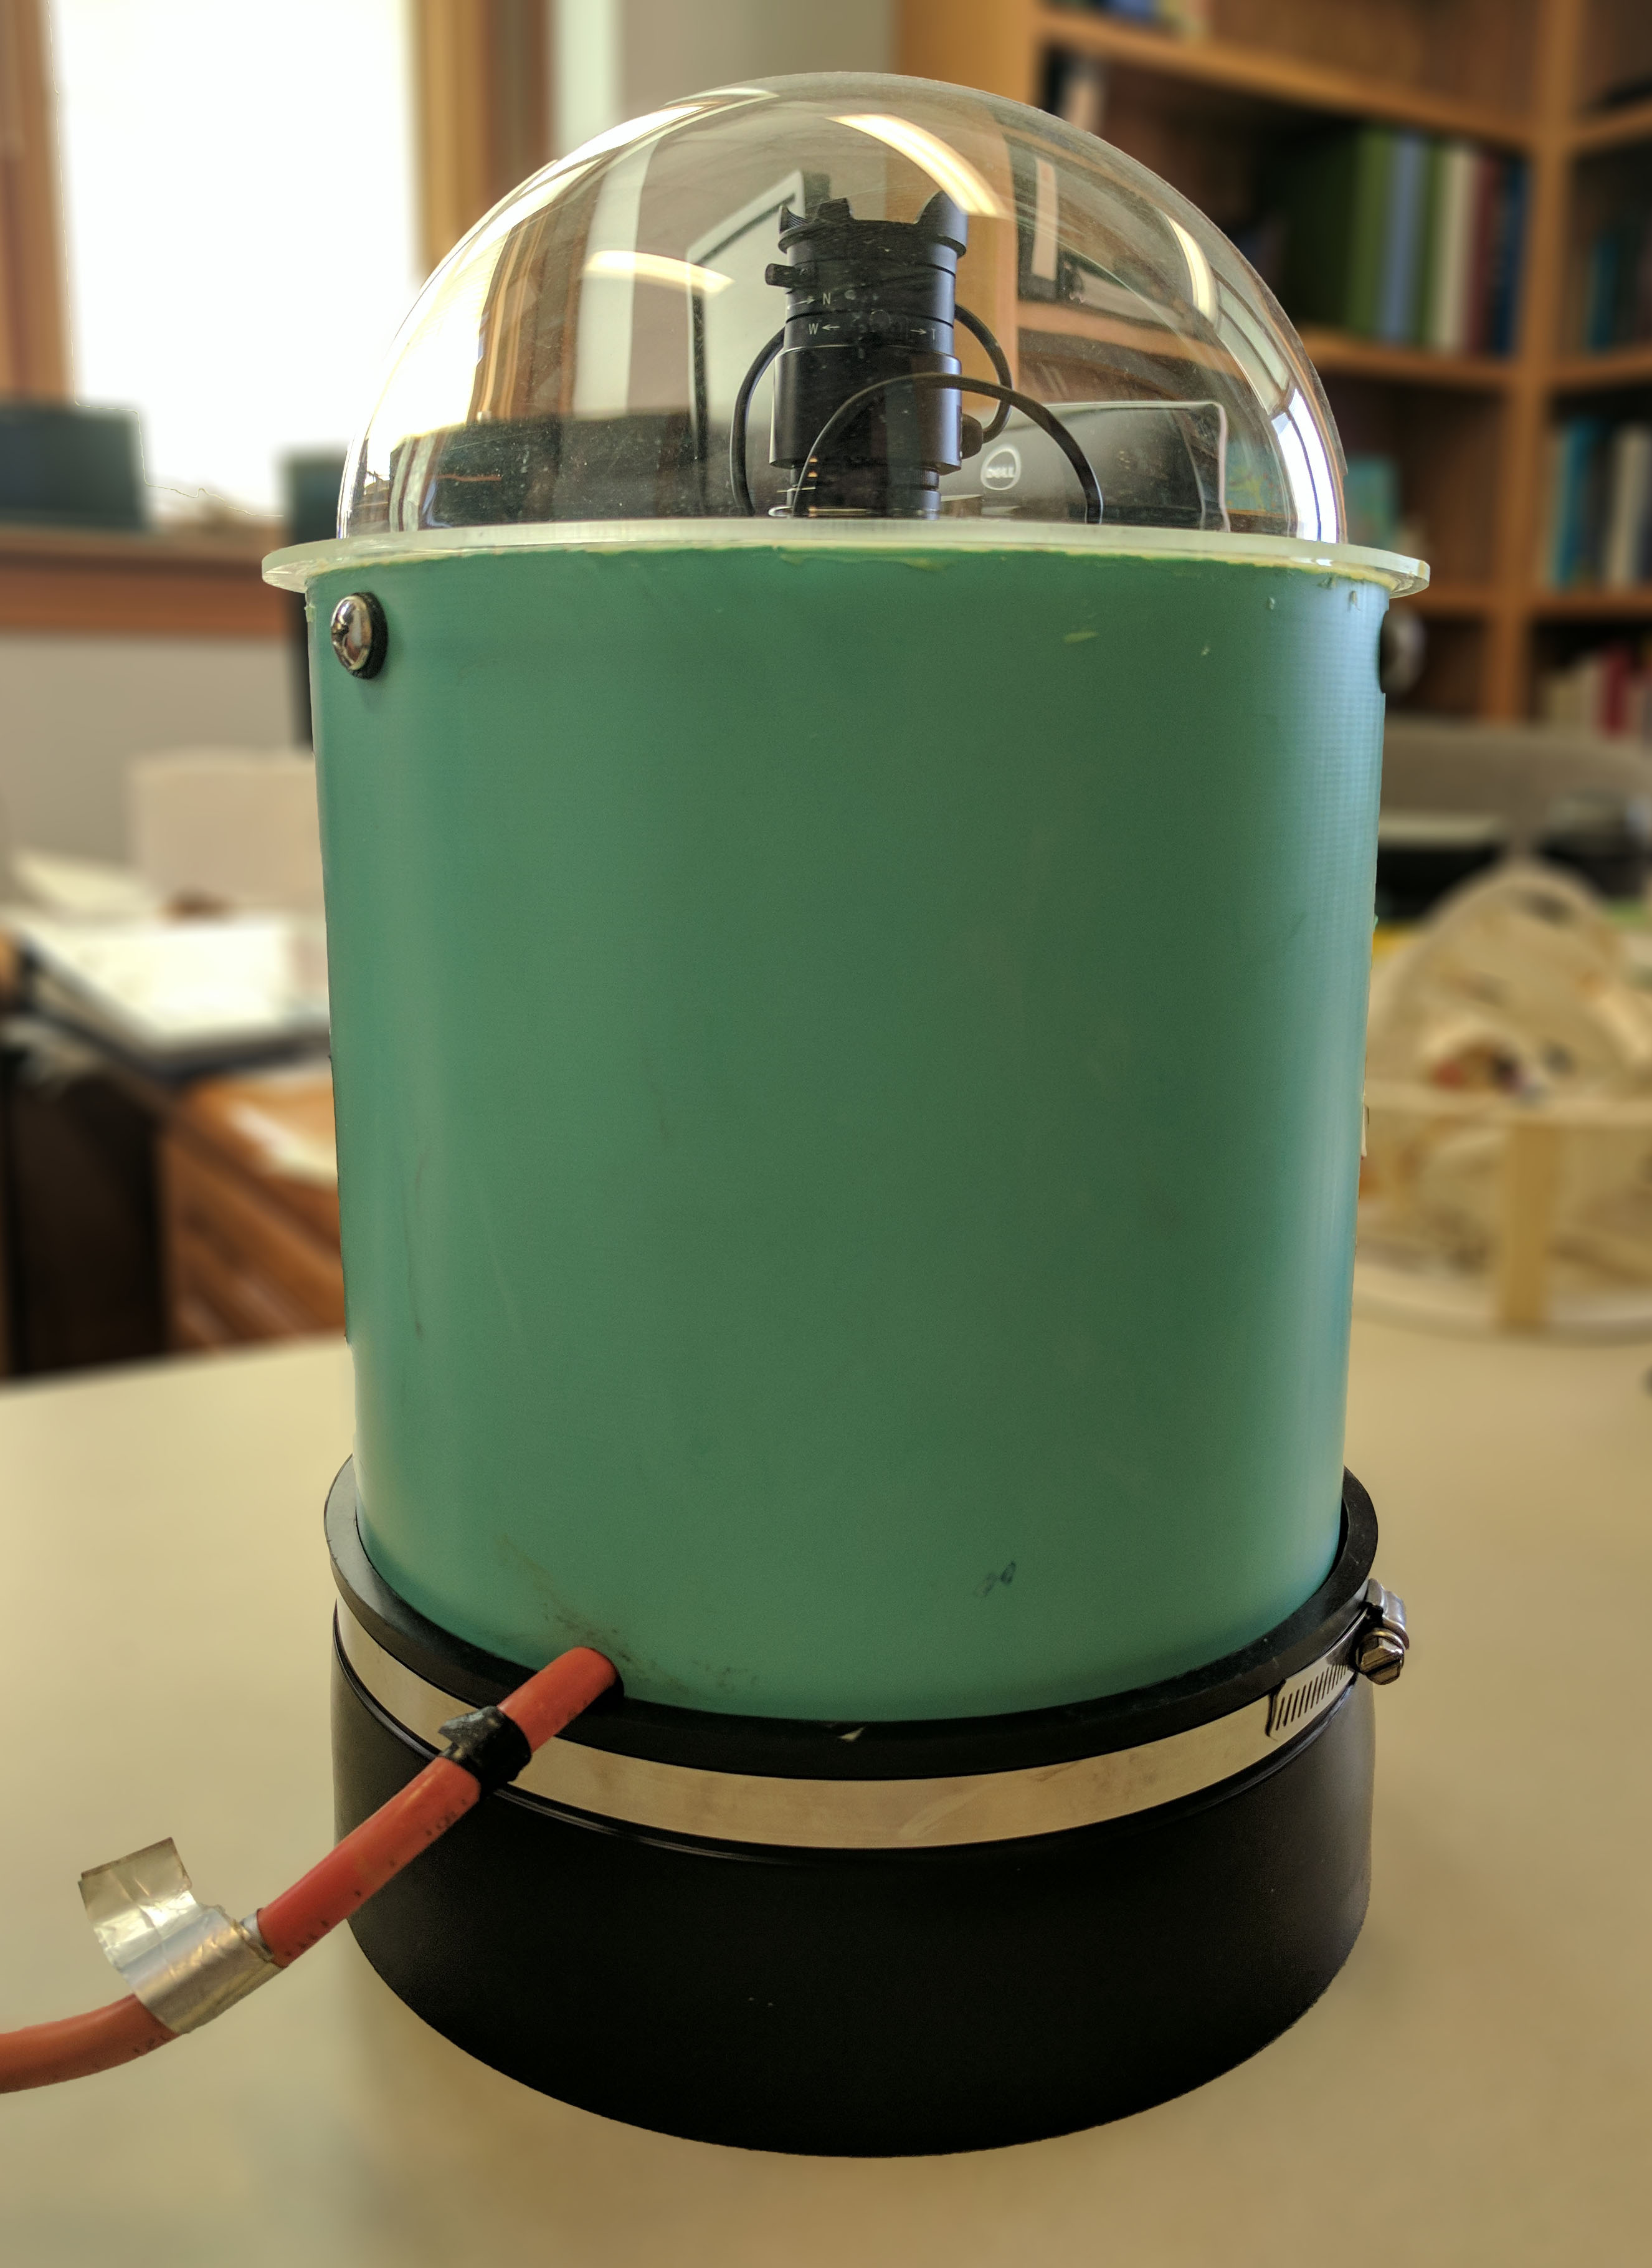
\includegraphics[height=6.5cm]{deesix.jpg}};
		\node<1> at (-5.25,-.5){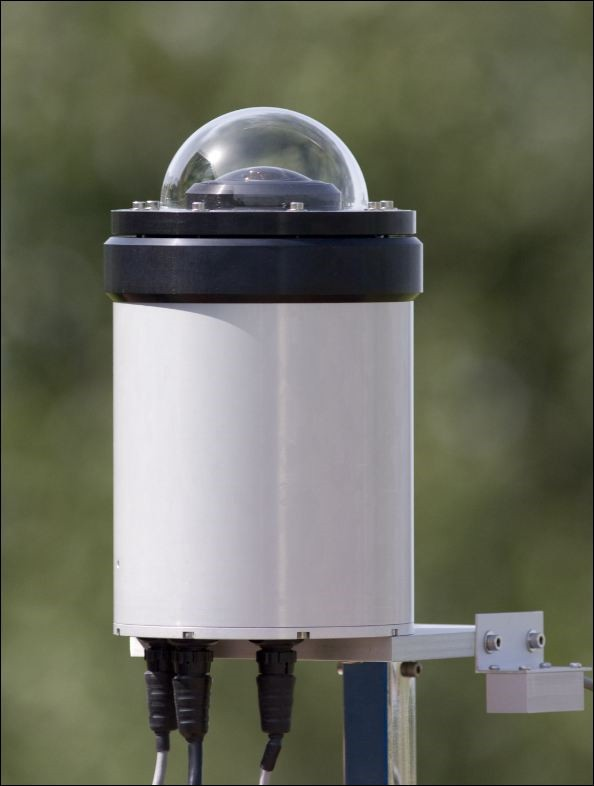
\includegraphics[height=6.5cm]{others.jpg}};
		\node<1> at (0,-.5){\includegraphics[height=6.5cm]{map.jpg}};
		\node<1> at (4.75,-1.7){
\includegraphics[height=4cm]{blank2.png}};
		\node<1> at (6.5,-2.6){Picture courtesy}; 
		\node<1> at (6.5,-3){of Alcor System};
	\end{tikzpicture}
\end{center}
%\end{figure}
%}
\end{frame}


%------------------------------------------------
\fbckg{skypic1.png}
\begin{frame}
\pgfsetfillopacity{.75}
\framedsl{All-Sky Cameras}
\pgfsetfillopacity{1}
	\begin{tikzpicture}[remember picture, overlay]
		\node<1> at (2.3,-4){
\includegraphics[height=4cm]{blank.png}};
		\node<1> at (.5,-2.7){Picture courtesy}; 
		\node<1> at (.5,-3.1){of Alcor System};
	\end{tikzpicture}
\end{frame}


%------------------------------------------------

%\fbckg{bw.jpg}
%\begin{frame}
%\pgfsetfillopacity{.75}
%\framedsl{Our All-Sky Camera}
%\pgfsetfillopacity{1}
	%\begin{tikzpicture}[remember picture, overlay]
		%\node<1> at (2.3,-4){
\includegraphics[height=4cm]{blank.png}};
		%\node<1> at (.5,-2.7){Picture courtesy}; 
		%\node<1> at (.5,-3.1){of SBIG};
	%\end{tikzpicture}
%\end{frame}

%------------------------------------------------
\fbckg{2.jpg} % Slide background image
\begin{frame}
	\pgfsetfillopacity{.75}
	\framedsl{from brightness to mass}
	\pgfsetfillopacity{1}
	\begin{center}
	
\includegraphics[width=\linewidth, height = 200pt]{chain.png}
	\end{center}
	\begin{tikzpicture}[remember picture, overlay]
		%\node at (0,0) {includegraphics[width=.8linewidth]{chain.png}}
		\node[font=\bf\LARGE] at (4.70,6.65) {$m = -2.5\log(I)$};
		\node[font=\bf\huge] at (9.5,4.25) {$L = \tau \frac{v^2}{2} \frac{dM}{dt}$};
		\node[math,font=\bf\LARGE] at (4.65,1.75) {M =\int \frac{2L}{\tau v^2}\,dt};

		\onslide<1>{
			\fill[black,opacity=0.5] (7.25,5.5) rectangle +(9,2.25);
			\node at (10,7.15) {$m$ = magnitude};
			\node at (10,6.65) {$I$ = sum of object's pixel values};
		}

		\onslide<1>{
			\fill[black,opacity=0.5] (-1,3.14) rectangle +(7,2.25);
			\node at (4,5) {$L$ = luminosity};
			\node at (4,4.6) {$v$ = velocity};
			\node at (4,4.2) {$M$ = mass};
			\node at (4,3.8) {$\tau$ = luminous efficiency};
			\node at (4,3.4) {$t$ = time};
		}


	\end{tikzpicture}
\end{frame}

%------------------------------------------------

%------------------------------------------------
%\fbckg{2.jpg} % Slide background image
%\begin{frame}
	%
\includegraphics[width=1\linewidth]{lightchain.png}
	%\begin{tikzpicture}[remember picture, overlay]
		%\node[font=\bf\LARGE] at (4.7,4.5) {$m = -2.5log(\frac{I}{I_o})$};
	%\end{tikzpicture}
%\end{frame}
%------------------------------------------------
% First slide of detection
%------------------------------------------------
\fbckg{bw.jpg} 
\begin{frame}
	\pgfsetfillopacity{.75}
	\framedsl{Determining magnitude}
	\pgfsetfillopacity{1}
	\begin{tikzpicture}[remember picture, overlay]
		\node<1,2,3> at (15,-4){
\includegraphics[width=.75\linewidth]{lightchain.png}};
		\node[font=\bf\LARGE] at (13.25,-3) {$-2.5\log(I)$};
  		\onslide<2-3>{
	  		\draw[line width=2pt,newhopeblue,opacity=.7] (4.85,2.68) circle (2mm);
		}		
		\onslide<3>{
			\draw[line width=2pt,newhopeblue,opacity=.7] (7.35,-1.3) circle (2mm);
		}
	\end{tikzpicture}
\end{frame}

%------------------------------------------------
% ---
%------------------------------------------------

\fbckg{2.jpg} % Slide background image
\begin{frame}
\pgfsetfillopacity{.75}
\framedsl{Raw Data}
\pgfsetfillopacity{1}
\begin{center}
	\begin{tikzpicture}[remember picture, overlay]
		\node<1> at (3.25,-.5){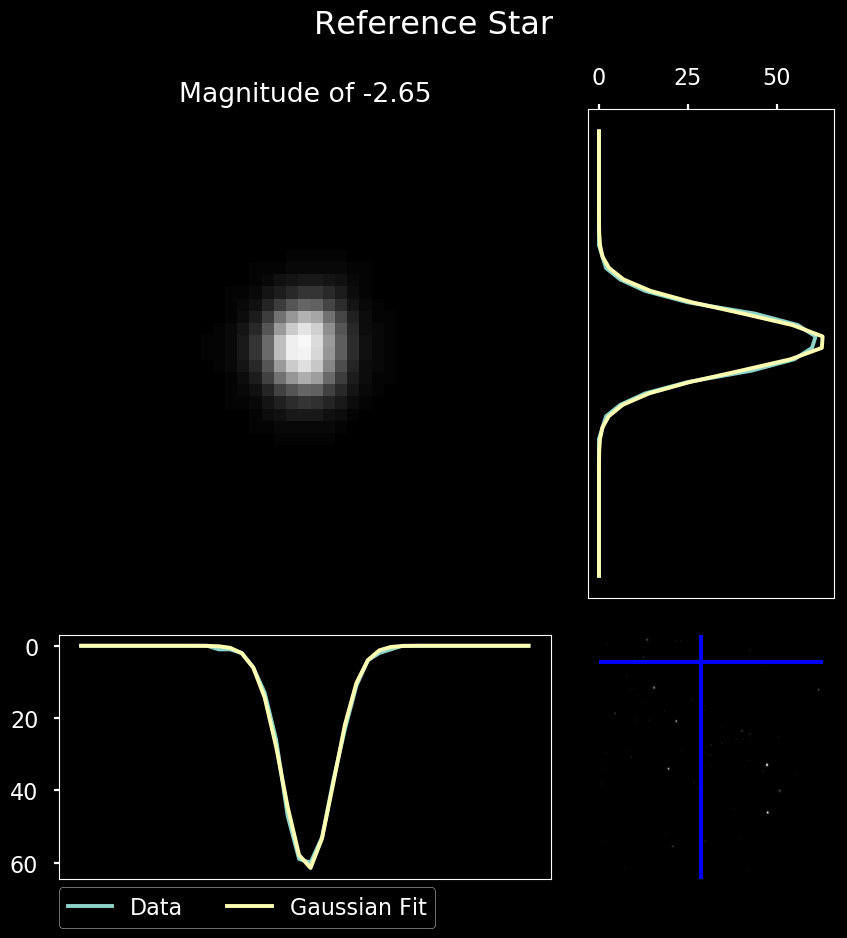
\includegraphics[height=6.5cm]{ReferencePlot.png}};
		\node<1> at (-3.25,-.5){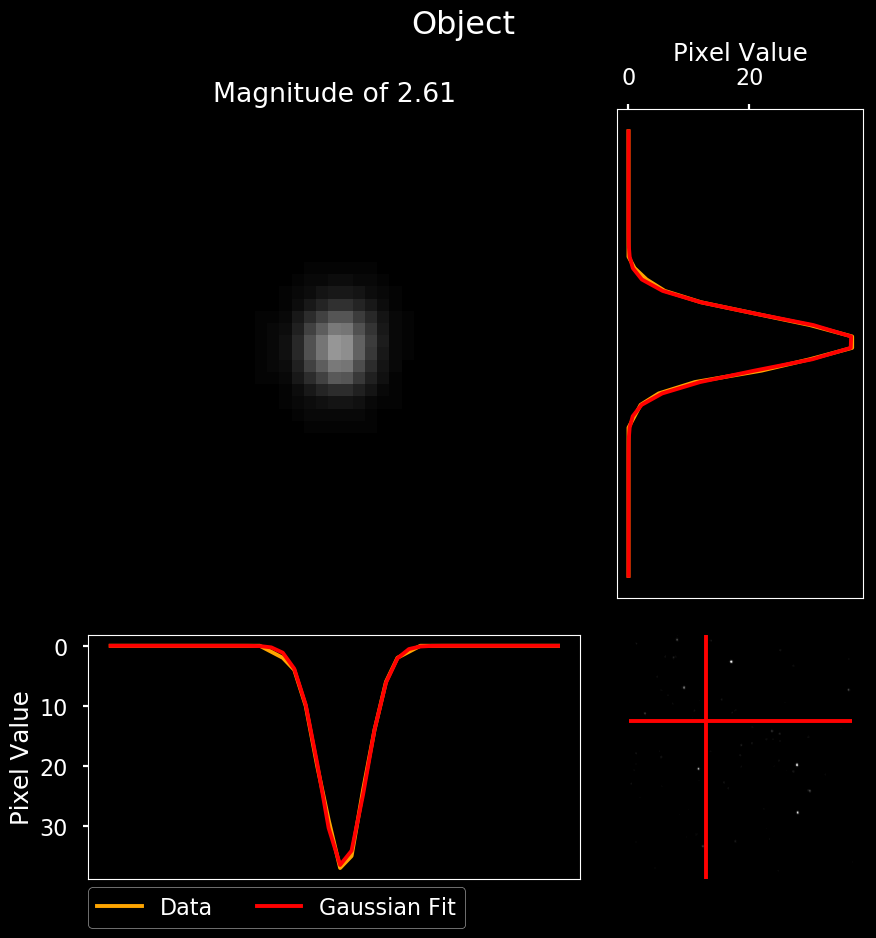
\includegraphics[height=6.5cm]{ObjectPlot.png}};
		%\node<1> at (4.75,-1.7){
\includegraphics[height=4cm]{blank2.png}};
		%\node<1> at (6.5,-2.6){Picture courtesy}; 
		%\node<1> at (6.5,-3){of Alcor System};
	\end{tikzpicture}
\end{center}
\end{frame}

%------------------------------------------------
\fbckg{2.jpg} % Slide background image
\begin{frame}
\pgfsetfillopacity{.75}
\framedsl{Raw Data}
\pgfsetfillopacity{1}
\begin{center}
	\begin{tikzpicture}[remember picture, overlay]
		\node<1> at (3.25,-.5){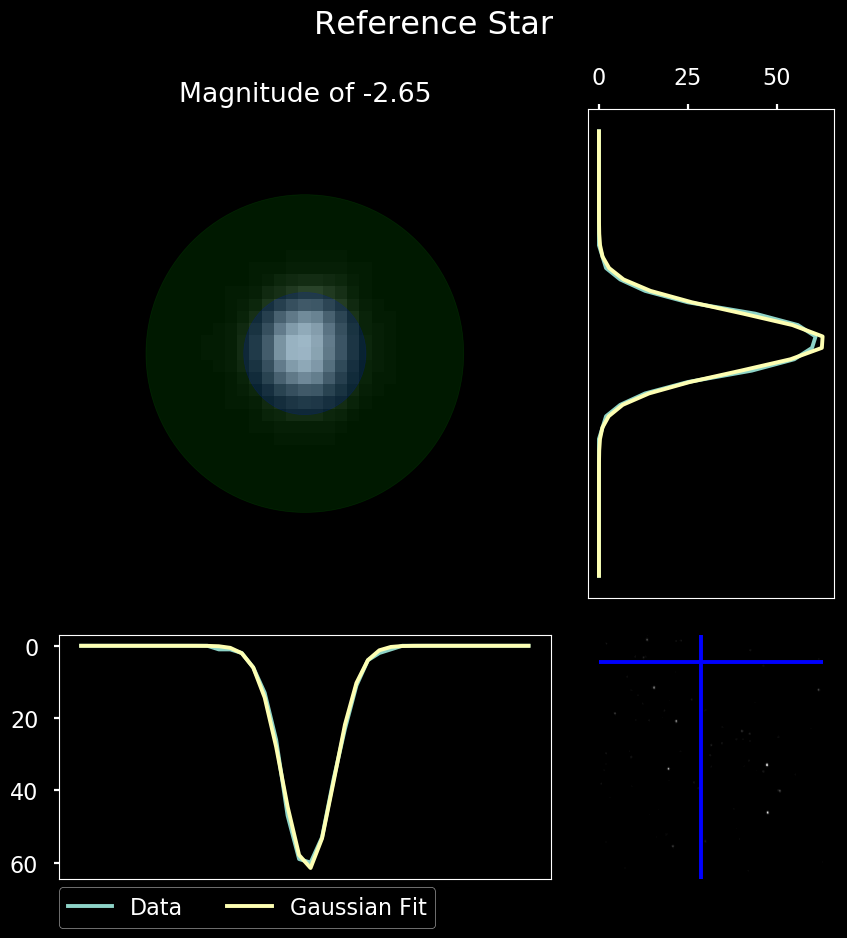
\includegraphics[height=6.5cm]{ReferencePlotCircle.png}};
		\node<1> at (-3.25,-.5){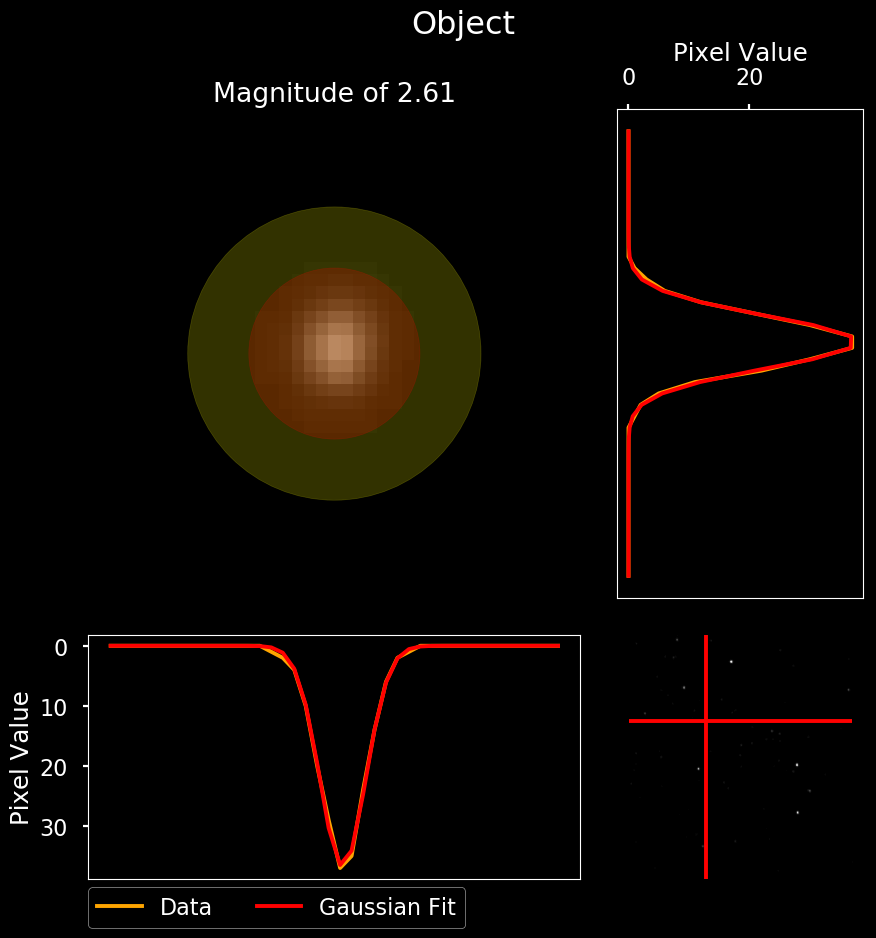
\includegraphics[height=6.5cm]{ObjectPlotCircle.png}};
		%\node<1> at (4.75,-1.7){
\includegraphics[height=4cm]{blank2.png}};
		%\node<1> at (6.5,-2.6){Picture courtesy}; 
		%\node<1> at (6.5,-3){of Alcor System};
	\end{tikzpicture}
\end{center}
\end{frame}


%------------------------------------------------
%\fbckg{2.jpg} % Slide background image
%\begin{frame}
	%\begin{tikzpicture}[remember picture, overlay]
		%\node<1> at (7,0){
\includegraphics[width=1.3\linewidth]{half2.png}};
		%\node<1> at (4,-2.5){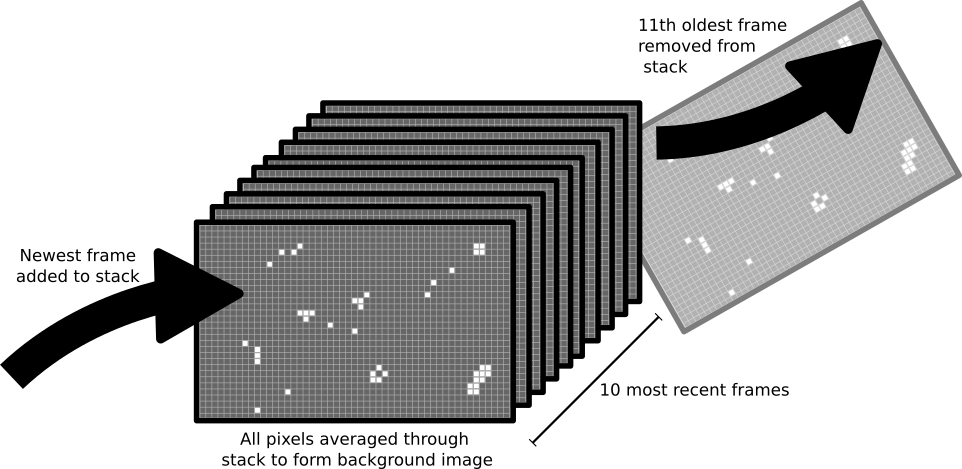
\includegraphics[width=.6\linewidth]{placehold.png}};
	%\end{tikzpicture}
%\end{frame}

%-----------------------------------------------
%\fbckg{iridium.png}
%\fbckg{iridium.png}
\begin{frame}
	%\fullFrameMovie{flare.avi}{iridium.png};
	\pgfsetfillopacity{.75}
	\framedsl{Iridium Flares}
	\pgfsetfillopacity{1}
	\center
	\inlineMovie{flare.ogv}{iridium.png}{width=11cm} 

	%\begin{tikzpicture}[remember picture, overlay]
          %\onslide<1>{
			%\node[anchor=south, outer sep=0pt, inner sep=0pt] at ($(current page.south)-(2,0)$) {\inlineMovie{flare.ogv}{iridium.png}{width=11cm} };
			%\node at (15,-4){
\includegraphics[width=.65\linewidth]{lightchain.png}};
			%\node[math,font=\bf\Large] at (13.4,-3.1) {-2.5 log(I)};
				%}

	%\end{tikzpicture}



\end{frame}

%------------------------------------------------
%\fbckg{iridium3.png} % Slide background image
%\begin{frame}
%\pgfsetfillopacity{.75}
%\framedsl{Iridium Flare: Photometric Data}
%\pgfsetfillopacity{1}
%\center
%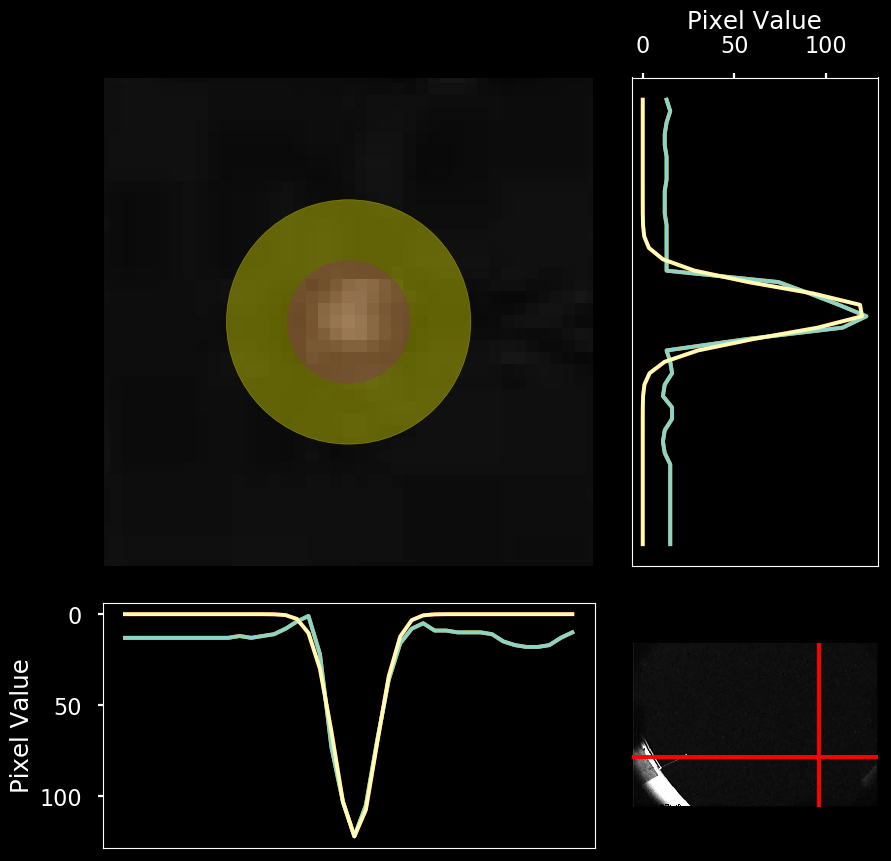
\includegraphics[width=.50\linewidth]{iridiumgraph1.png}
%\end{frame}


%------------------------------------------------

%\fbckg{iridium3.png} % Slide background image
%\begin{frame}
%\pgfsetfillopacity{.75}
%\framedsl{Irdium Flare: Light Curve}
%\pgfsetfillopacity{1}
%\center
%\includegraphics[width=.50\linewidth]{iridiumlightcurve.png}
%\end{frame}

%------------------------------------------------

\fbckg{iridium3.png} % Slide background image
\begin{frame}
\pgfsetfillopacity{.75}
\framedsl{Iridium Flare: Light Curve}
\pgfsetfillopacity{1}
\begin{center}
	\begin{tikzpicture}[remember picture, overlay]
		\fill[newhopeblue,opacity=0] ($(current page.west)+(0,3.5)$) rectangle +(20,-7);
		\node<1> at (3.75,-.5){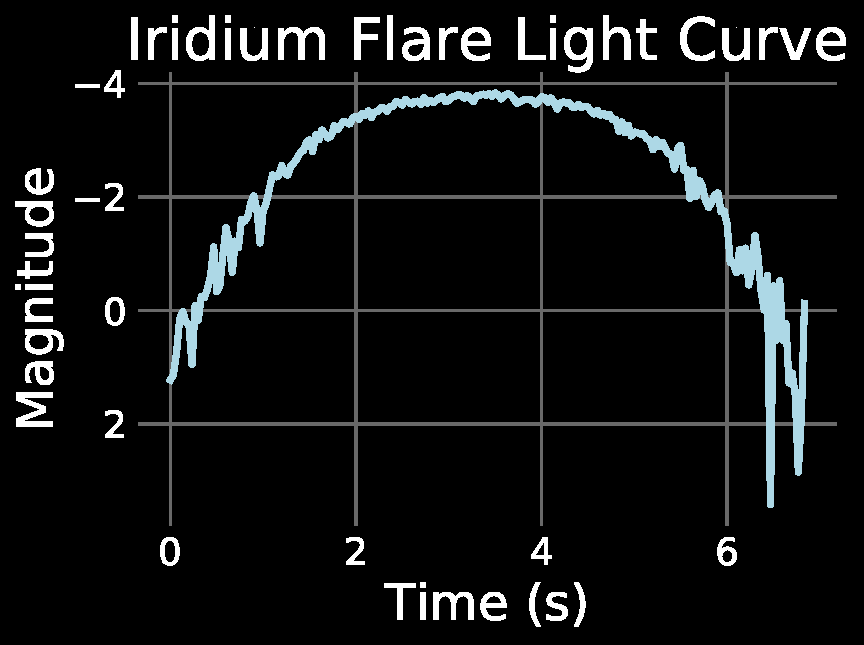
\includegraphics[height=5.5cm]{IridiumCurve.pdf}};
		\node<1> at (-3.75,-.5){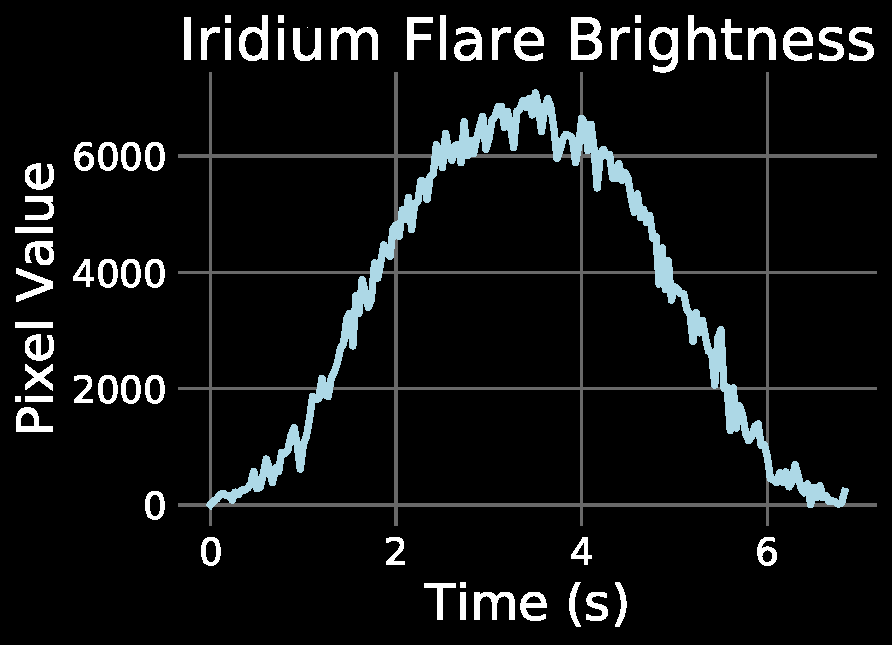
\includegraphics[height=5.5cm]{IridiumMag.pdf}};
	\end{tikzpicture}
\end{center}
\end{frame}



%------------------------------------------------
\fbckg{2.jpg}
\begin{frame}
	\pgfsetfillopacity{.75}
	\framedsl{NASA Meteors}
	\pgfsetfillopacity{1}
	\center
	\inlineMovie{NASA.ogv}{NASAPicture.png}{width=9.75cm}

	%\begin{tikzpicture}[remember picture, overlay]
          %\onslide<1>{
			%\node[anchor=south, outer sep=0pt, inner sep=0pt] at ($(current page.south)-(2,-.1)$) {\inlineMovie{NASA.ogv}{NASAPicture.png}{width=10cm} };
			%\node at (15,-4){
\includegraphics[width=.65\linewidth]{lightchain.png}};
			%\node[math,font=\bf\Large] at (13.4,-3.1) {-2.5 log(I)};

		%}

	%\end{tikzpicture}

\end{frame}

%-------------------------------------------------
%\fbckg{nasastill.png} % Slide background image
%\begin{frame}
%\pgfsetfillopacity{.75}
%\framedsl{NASA Meteor: Photometric Data}
%\pgfsetfillopacity{1}
%\center
%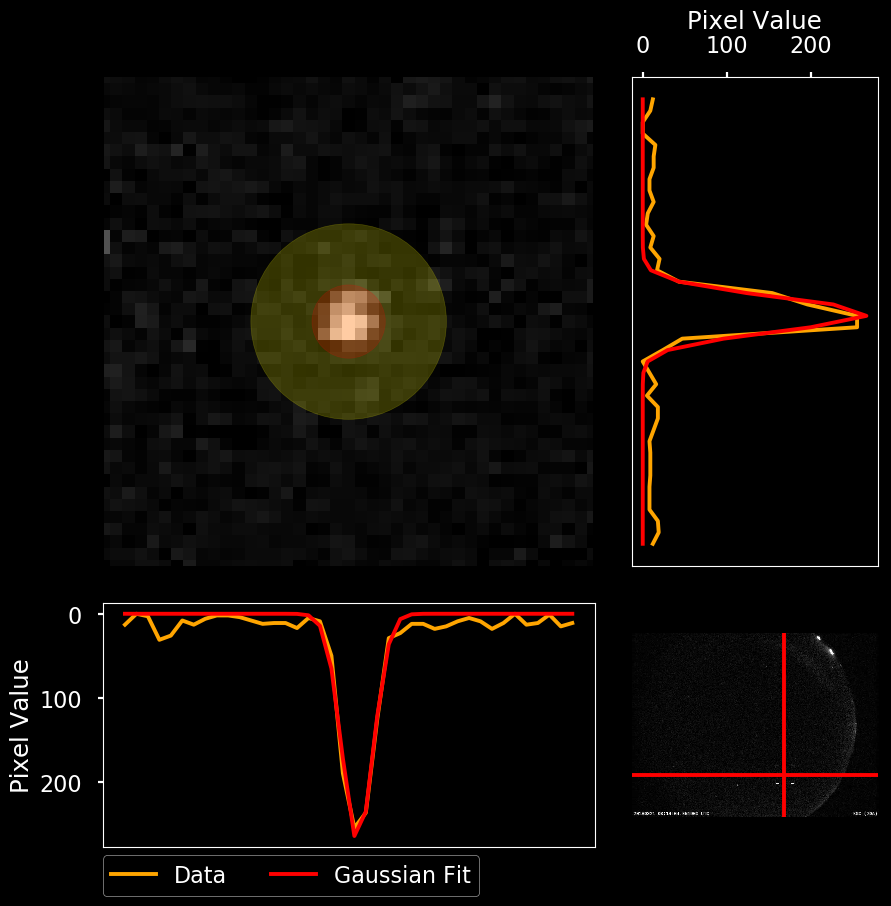
\includegraphics[width=.50\linewidth]{NASAPlot.png}
%\end{frame}


%------------------------------------------------
\fbckg{nasastill.png} % Slide background image
\begin{frame}
\pgfsetfillopacity{.75}
\framedsl{NASA Meteor: Light Curve}
\pgfsetfillopacity{1}
\center
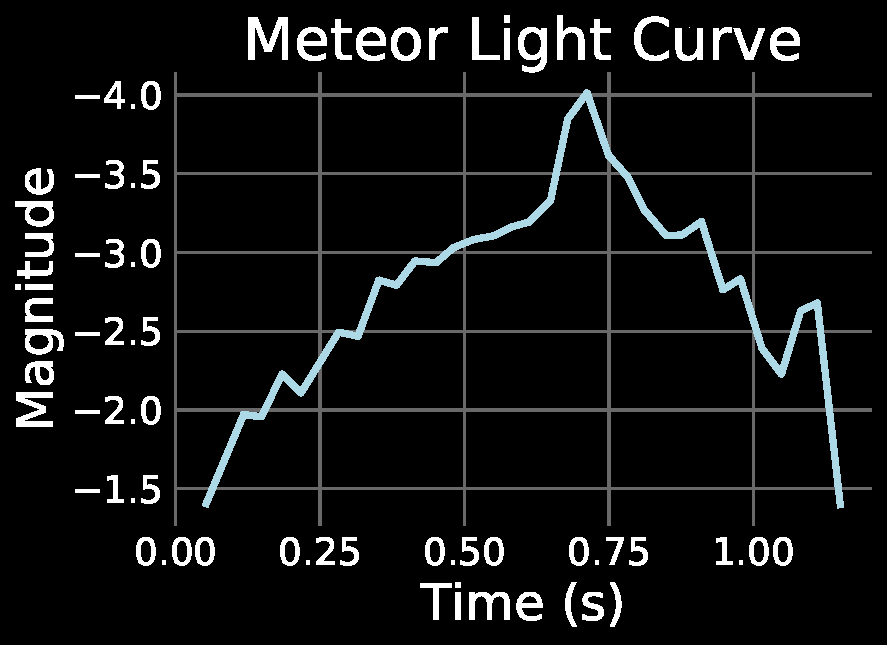
\includegraphics[width=.65\linewidth]{MeteorCurve.pdf}
\end{frame}

%-----------------------------------------------

\fbckg{nasastill.png} % Slide background image
\begin{frame}
\pgfsetfillopacity{.75}
\framedsl{NASA Meteor: Light Curve}
\pgfsetfillopacity{1}
\center
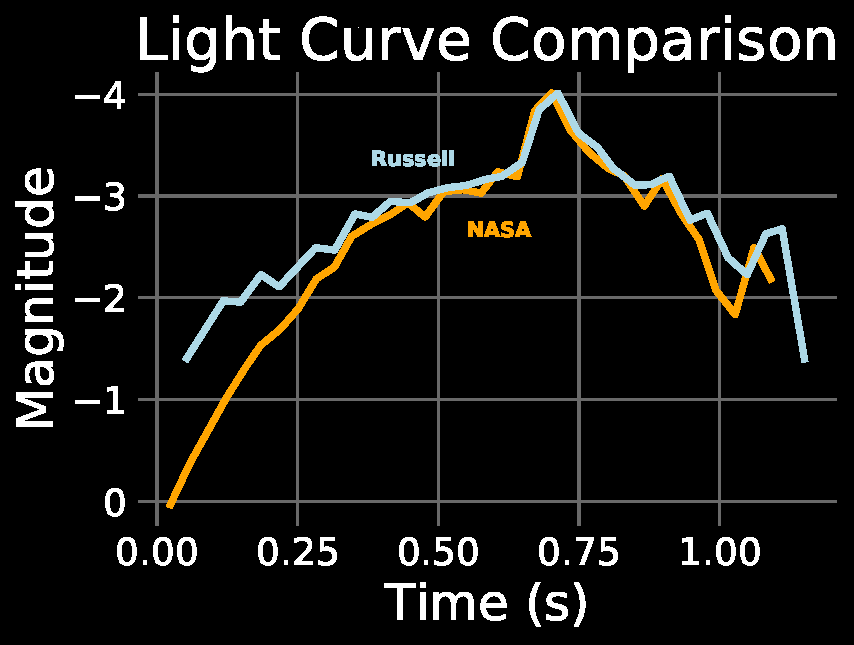
\includegraphics[width=.65\linewidth]{LightComparison0.pdf}
\end{frame}

%------------------------------------------------

\fbckg{nasastill.png} % Slide background image
\begin{frame}
%\misc{ % Anything can be placed inside the \misc{} command
%\begin{figure}[h
\pgfsetfillopacity{.75}
\framedsl{NASA Meteors: Light Curves}
\pgfsetfillopacity{1}
\begin{center}
	\begin{tikzpicture}[remember picture, overlay]
		\fill[newhopeblue,opacity=0] ($(current page.west)+(0,3.5)$) rectangle +(20,-7);
		\node<1> at (2.75,-2.5){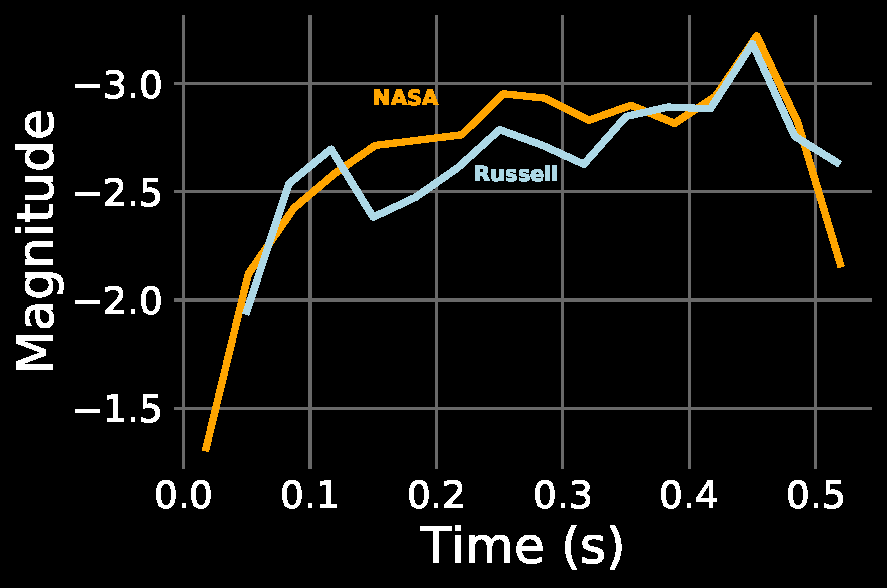
\includegraphics[width=5.1cm,height=3.5cm]{Comparison5.pdf}};
		\node<1> at (2.75,1.25){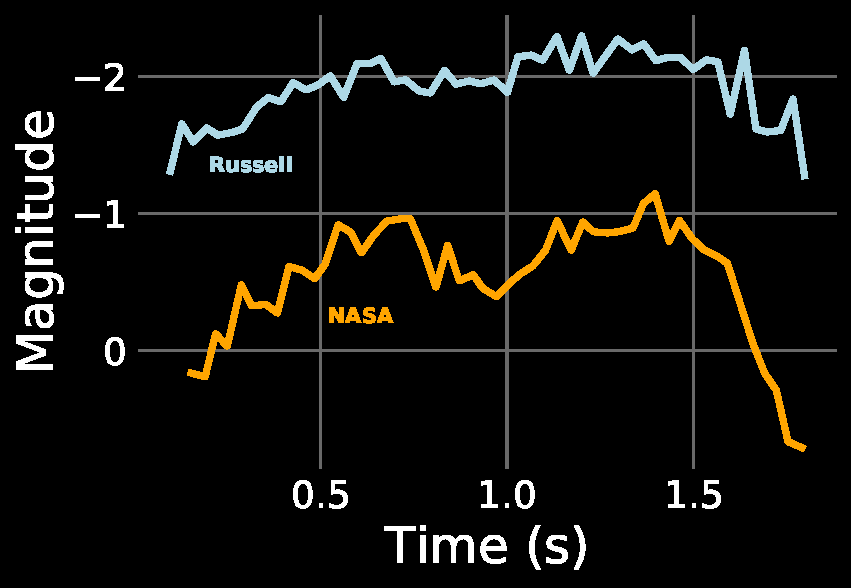
\includegraphics[width=5.1cm,height=3.5cm]{Comparison2.pdf}};
		\node<1> at (-2.75,-2.5){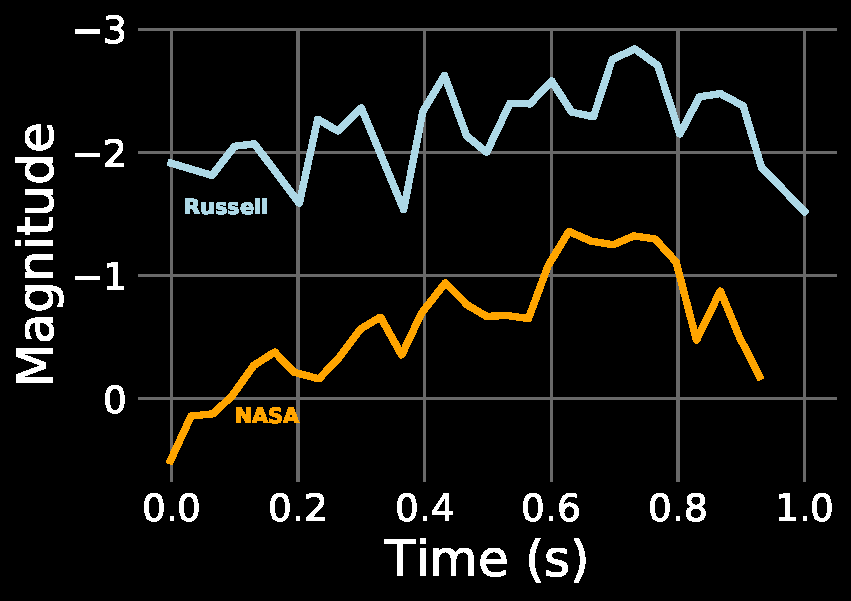
\includegraphics[width=5.1cm,height=3.5cm]{Comparison3.pdf}};
		\node<1> at (-2.75,1.25){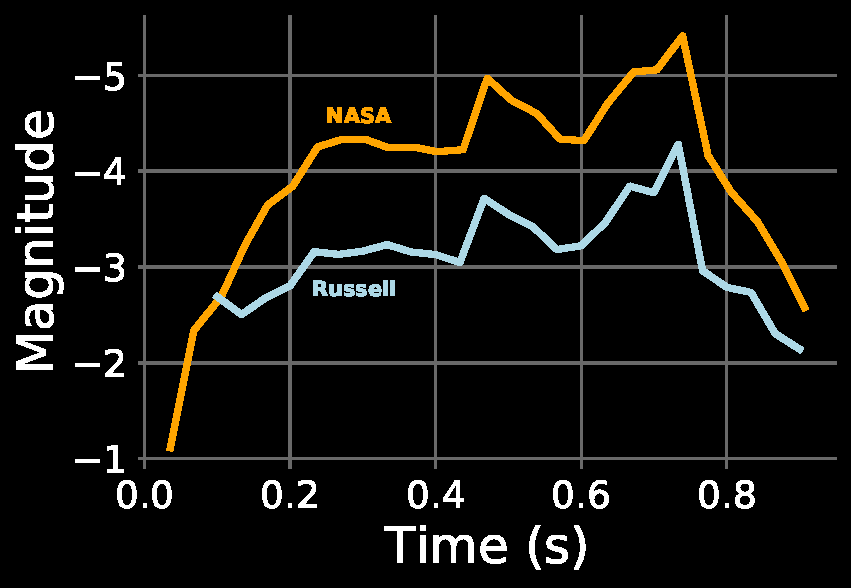
\includegraphics[width=5.1cm,height=3.5cm]{Comparison4.pdf}};
	\end{tikzpicture}
\end{center}
%\end{figure}
%}
\end{frame}


%------------------------------------------------
%------------------------------------------------
\fbckg{2.jpg}
\begin{frame}
	\pgfsetfillopacity{.75}
	\framedsl{D6 Fireballs}
	\pgfsetfillopacity{1}
	\center
	\inlineMovie{Fireball.ogv}{fireballscreenshot.png}{width=10.5cm}

	%\begin{tikzpicture}[remember picture, overlay]
          %\onslide<1>{
			%\node[anchor=south, outer sep=0pt, inner sep=0pt] at ($(current page.south)-(2,-.5)$) {\inlineMovie{Fireball.ogv}{fireballscreenshot.png}{width=10cm} };
			%\node at (15,-4){
\includegraphics[width=.65\linewidth]{lightchain.png}};
			%\node[math,font=\bf\Large] at (13.4,-3.1) {-2.5 log(I)};
		%}

	%\end{tikzpicture}
\end{frame}
%------------------------------------------------
\fbckg{iridium3.png} % Slide background image
\begin{frame}
\pgfsetfillopacity{.75}
\framedsl{D6: Photometric Data}
\pgfsetfillopacity{1}
\begin{center}
	\begin{tikzpicture}[remember picture, overlay]
		\fill[newhopeblue,opacity=0] ($(current page.west)+(0,3.5)$) rectangle +(20,-7);
		\node<1> at (3,-.5){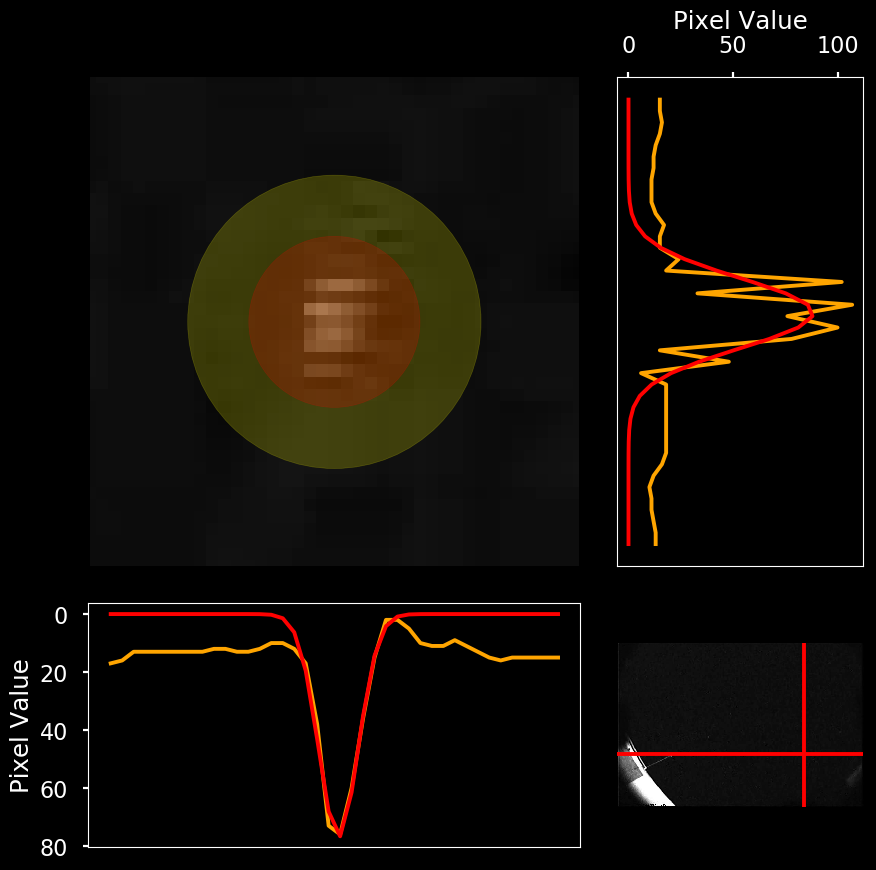
\includegraphics[height=5.5cm]{D6Glitch.png}};
		\node<1> at (-3,-.5){\includegraphics[height=5.5cm]{D6Good.png}};
	\end{tikzpicture}
\end{center}
\end{frame}

%------------------------------------------------
\fbckg{iridium3.png} % Slide background image
\begin{frame}
\pgfsetfillopacity{.75}
\framedsl{D6: Light Curve}
\pgfsetfillopacity{1}
\center
\includegraphics[width=.7\linewidth]{D6Curve.pdf}
\end{frame}

%------------------------------------------------


%\fbckg{iridium.png}
%\begin{frame}
	%\pgfsetfillopacity{.75}
	%\framedsl{Moving Targets: Meteor Showers}
	%\pgfsetfillopacity{1}
	%\begin{tikzpicture}[remember picture, overlay]
		%\onslide<1>{	
			%\fill[white,opacity=0.3] (-1,3.14) rectangle +(22,-9);
		%}	
		%%\node<1> at (7,-.5){\includegraphics[width=.8\linewidth]{shower.png}};
		%\node<1> at (7,-.75){\inlineMovie{moving1.ogv}{shower.png}{width=9.5cm} };
		%\node<1> at (2.3,-4){\includegraphics[height=4cm]{blank.png}};
		%\node<1> at (.5,-2.7){Picture courtesy}; 
		%\node<1> at (.5,-3.1){meteorshower.com};

		%\node<1> at (11.75,3){\includegraphics[height=4cm]{blank2.png}};
		%\node<1> at (13.5,2.2){The Geminids}; 
		%\node<1> at (13.5,1.75){December 15};
	%\end{tikzpicture}


%\end{frame}

%-----------------------------------------------
\fbckg{2.jpg} % Slide background image
\begin{frame}
	\pgfsetfillopacity{.75}
	\framedsl{from brightness to mass}
	\pgfsetfillopacity{1}
	\begin{center}
	\includegraphics[width=\linewidth, height = 200pt]{chain.png}
	\end{center}
	\begin{tikzpicture}[remember picture, overlay]
		%\node at (0,0) {includegraphics[width=.8linewidth]{chain.png}}
		\node[font=\bf\LARGE] at (4.70,6.65) {$m = -2.5\log(I)$};
		\node[font=\bf\huge] at (9.5,4.25) {$L = \tau \frac{v^2}{2} \frac{dM}{dt}$};
		\node[math,font=\bf\LARGE] at (4.65,1.75) {M =\int \frac{2L}{\tau v^2}\,dt};

		\fill[black,opacity=0.5] (7.25,5.5) rectangle +(9,2.25);
		\node at (10,7.15) {$m$ = magnitude};
		\node at (10,6.65) {$I$ = sum of object's pixel values};

		\fill[black,opacity=0.5] (-1,3.14) rectangle +(7,2.25);
		\node at (4,5) {$L$ = luminosity};
		\node at (4,4.6) {$v$ = velocity};
		\node at (4,4.2) {$M$ = mass};
		\node at (4,3.8) {$\tau$ = luminous efficiency};
		\node at (4,3.4) {$t$ = time};
		\onslide<2>{
			\fill[black,opacity=0.7] (-2,5.55) rectangle +(20,2.3);
		}

	\end{tikzpicture}
\end{frame}


%-----------------------------------------------
\fbckg{2.jpg} % Slide background image
\begin{frame}
\pgfsetfillopacity{.75}
\framedsl{Long-Term Goal}
\pgfsetfillopacity{1}
\begin{center}
	\begin{tikzpicture}[remember picture, overlay]
		\fill[newhopeblue,opacity=0] ($(current page.west)+(0,3.5)$) rectangle +(20,-7);
		\node<1> at (0,-.5){\includegraphics[height=7cm]{populationdark.png}};
		\node<1> at (-4.75,-4){\includegraphics[height=4cm]{blank.png}};
		\node<1> at (-6.5,-2.7){Graph made by}; 
		\node<1> at (-6.5,-3.1){Dr. J. Rembold};
	\end{tikzpicture}
\end{center}
\end{frame}



%-----------------------------------------------



\fbckg{2.jpg}
\begin{frame}
	\pgfsetfillopacity{.75}
	\framedsl{References}
	\pgfsetfillopacity{1}
	\center
	\begin{itemize}
		\item Background picture 1: alcor-system.com
		\item Background picture 2: sbig.com
		\item Whitehead, James. ”The North American All-Sky Camera
Database.” (2009).
		\item Suggs, Rob M. ”The NASA Fireball Network All-Sky
Cameras.” (2011). 
		\item All icons made by Freepik
	\end{itemize}
\end{frame}

%-------------------------------------------------

\fbckg{2.jpg} % Slide background image
\begin{frame}
	\begin{tikzpicture}[remember picture, overlay]
		\node<1> at (7,0){\includegraphics[width=1.3\linewidth]{thanksblue.png}};
	\end{tikzpicture}
\end{frame}

%\fbckg{blank} % A blank background can be used instead of an image
%\begin{frame}
%\sources{ % An environment for giving credit for slide backgrounds, images will need to be scaled down if there are more than two
%\includegraphics[scale=0.048]{1.jpg} \ flickr/lovelornpoets\\
%\includegraphics[scale=0.2]{2.jpg} \ flickr/apsmuseum
%}
%\end{frame}

%----------------------------------------------------------------------------------------

\end{document}
